A computational mesh can be structured or unstructured and 
the choice of the element that constitutes this mesh is of 
vital importance for a good accuracy of the solution. 
Some parameters can influence the choice of a certain elements group, 
for instance in the case where there is a restriction condition 
as found in the Navier-Stokes equation due to the strong coupling 
between velocity and pressure fields. 
This restriction is known as \textit{Babuska-Brezzi} 
\cite{babuska1971} \cite{brezzi1974}. 
When we have this restriction, 
we need to have different numbers of nodes for each unkowns 
in the same element in order to have stability in the solution.
Therefore, we need to use a \textit{quadratic or cubic element}. 
This methodology is known as \textit{Mixed Finite Element Method}. 
But the vorticity-streamfunction formulation sstisfies 
the \textit{Babuska-Brezzi} restriction since there is no coupling 
between velocity and pressure. 
Thus, the use of a \textit{linear element} does not produce 
instability and can be used without problems in this work.

\medskip
Some triangular elements are presented with different orders of the interpolator polynomial below:

\medskip
\noindent
\textbf{Linear Triangular Element:} 
Due to its simplicity, 
it is the element most commonly used element in FEM when 
we have no restrictions. The analytical elementary matrices 
of this element are easily found in the literature. 
Since it is a linear element, the interpolation
polynomial is first order. 
In this way, its interpolation functions are plane. 
This element is represented by the \ref{elemento triangular linear}:


\begin{figure}[H]
\begin{center}
\begin{tikzpicture}[scale=3]
 \draw (0,0) -- (1,0) -- (0.5,1) -- cycle;

 \node[circle, fill=black, inner sep=0pt, minimum size=5pt,label=below left:{1}] at (0,0) {};
 \node[circle, fill=black, inner sep=0pt, minimum size=5pt,label=below right:{2}] at (1,0) {};
 \node[circle, fill=black, inner sep=0pt, minimum size=5pt,label=above:{3}] at (0.5,1) {};
 
 \node[draw=none, scale=1.2] at (2,0.5) {$N_i = L_i$};
 \node[draw=none, scale=1.2] at (3.2,0.5) {$i = 1,2,3$};
\end{tikzpicture}
\end{center}
\caption{Linear Triangular Element}
\label{elemento triangular linear}
\end{figure}

%\begin{figure}[H]
%  \centering
%  \includegraphics[scale=0.25]{./02_chaps/cap_mef/figure/tri_linear.png}
% \caption{Funções de Interpolação para o elemento triangular linear.}
% \label{tri_linear}
%\end{figure}


\medskip
\noindent
\textbf{Quad Triangular Element:} 
This element is generally used when we have restrictions that prevent 
the use of the linear element or when we are interested in 
a better accuracy of the result. The elementary matrices of 
this element are calculated using the Gaussian Quadrature 
whose parameters can be found in the literature. 
Since it is a quadratic element, the interpolation polynomial is
second order. 
In this way, its interpolation functions are parabolic. 
This element is represented by
\ref{elemento triangular quadrático}:

\begin{figure}[H]
\begin{center}
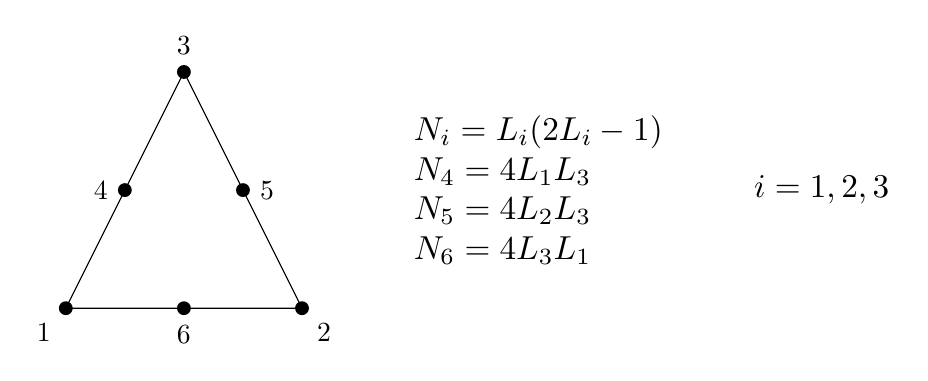
\begin{tikzpicture}[scale=3] 
 \draw (0,0) -- (1,0) -- (0.5,1) -- cycle;
 \node[circle, fill=black, inner sep=0pt, minimum size=5pt,label=below left:{1}] at (0,0) {};
 \node[circle, fill=black, inner sep=0pt, minimum size=5pt,label=below right:{2}] at (1,0) {};
 \node[circle, fill=black, inner sep=0pt, minimum size=5pt,label=above:{3}] at (0.5,1) {};
 \node[circle, fill=black, inner sep=0pt, minimum size=5pt,label=left:{4}] at (0.25,0.5) {};
 \node[circle, fill=black, inner sep=0pt, minimum size=5pt,label=right:{5}] at (0.75,0.5) {};
 \node[circle, fill=black, inner sep=0pt, minimum size=5pt,label=below:{6}] at (0.5,0.0) {};

 \node[draw=none, align=left, scale=1.2] at (2,0.5) {$N_i = L_i(2L_i - 1)$\\
                                                    $N_4 = 4L_1L_3$\\
                                                    $N_5 = 4L_2L_3$\\
                                                    $N_6 = 4L_3L_1$};

 \node[draw=none, scale=1.2] at (3.2,0.5) {$i = 1,2,3$};
\end{tikzpicture}
\end{center}
\caption{Quad Triangular Element}
\label{elemento triangular quadrático}
\end{figure}

\medskip
\noindent
\textbf{Mini Triangular Element:} 
This element is used when we have restrictions that 
prevent the use of the linear element or when we are interested in 
a better accuracy of the result as well as quad element. 
Their elementary matrices are also calculated using 
the Gaussian Quadrature. Although it is an incomplete cubic element, 
the interpolation polynomial is still of third order. 
In this way, its interpolation functions have a bubble in the center 
of the element. This element is represented by
\ref{elemento triangular mini}:

\begin{figure}[H]
\begin{center}
\begin{tikzpicture}[scale=3] 
 \draw (0,0) -- (1,0) -- (0.5,1) -- cycle;
 \node[circle, fill=black, inner sep=0pt, minimum size=5pt,label=below left:{1}] at (0,0) {};
 \node[circle, fill=black, inner sep=0pt, minimum size=5pt,label=below right:{2}] at (1,0) {};
 \node[circle, fill=black, inner sep=0pt, minimum size=5pt,label=above:{3}] at (0.5,1) {};
 \node[circle, fill=black, inner sep=0pt, minimum size=5pt,label=above:{4}] at (1/2,1/3) {};
 
 \node[draw=none, align=left, scale=1.2] at (2,0.5) {$N_i = L_1 - 9L_1L_2L_3$\\
                                                    $N_4 = 27L_1L_2L_3$};

 \node[draw=none, scale=1.2] at (3.2,0.5) {$i = 1,2,3$};
\end{tikzpicture}
\end{center}
\caption{Mini Triangular Element}
\label{elemento triangular mini}
\end{figure}





%\begin{figure}[H]
%  \centering
%  \includegraphics[scale=0.25]{./02_chaps/cap_mef/figure/mini.png}
% \caption{Funções de Interpolação para o elemento MINI.}
% \label{mini}
%\end{figure}

\medskip
Triangular elements are the most common in 2D-FE Method because 
it allows a good discretization of irregular surfaces 
due to its geometric simplicity. In this work, we use a triangular 
element with the interpolator polynomial of order one, that is, linear.
Therefore, 
the Eqs (\ref{vorticity pre matrix} to \ref{concentration pre matrix})
can be represented in matrix form by:

\begin{equation}
\begin{aligned}
 M \overset{.}{w} + u \cdot G_x w  + v \cdot G_y w & + \frac{1}{\textit{Re}} \Big[ K_{xx} + K_{yy} \Big] w
 \\[5pt]
 & + \frac{\Delta t}{2} u \Big[ u K_{xx} + v K_{yx} \Big] w 
 + \frac{\Delta t}{2} v \Big[ u K_{xy} + v K_{yy} \Big] w 
 = 0 \label{vorticity matrix}
\end{aligned}
\end{equation}

\begin{equation}
 - \Big[ K_{xx} + K_{yy} \Big] \psi + Mw = 0
\end{equation}

\begin{equation}
 Mu - G_y \psi = 0
\end{equation}

\begin{equation}
 Mv + G_x \psi = 0
\end{equation}

\begin{equation}
\begin{aligned}
 M \overset{.}{c} + u \cdot G_x c + v \cdot G_y c & + \frac{1}{\textit{ReSc}} \Big[ K_{xx} + K_{yy} \Big] c
 \\[5pt]
 & + \frac{\Delta t}{2} u \Big[ u K_{xx} + v K_{xy} \Big] c
 + \frac{\Delta t}{2} v \Big[ u K_{yx} + v K_{yy} \Big] c 
 = 0 \label{concentration matrix}
\end{aligned} 
\end{equation}

\medskip
\noindent
where the \textbf{M}, \textbf{G\textsubscript{x}}, 
\textbf{G\textsubscript{y}}, \textbf{K\textsubscript{xx}},
\textbf{K\textsubscript{xy}},
\textbf{K\textsubscript{yx}}, 
\textbf{K\textsubscript{yy}} matrices
have \textbf{np} x \textbf{np} size
(where \textit{np} is node number) and
they are defined as:

\begin{align}
  \textbf{M} & = \textbf{A} m^{e}\\
  \textbf{G\textsubscript{x}} & = \textbf{A} g_{x}^{e}\\
  \textbf{G\textsubscript{y}} & = \textbf{A} g_{y}^{e} \\
  \textbf{K\textsubscript{xx}} & = \textbf{A} k_{xx}^{e} \\
  \textbf{K\textsubscript{xy}} & = \textbf{A} k_{xy}^{e} \\
  \textbf{K\textsubscript{yx}} & = \textbf{A} k_{yx}^{e} \\
  \textbf{K\textsubscript{yy}} & = \textbf{A} k_{yy}^{e}
\end{align}

\noindent
where \textbf{A} is an assembly operator
that it assembles the elementary matrix in
global matrix, satisfying the local and global matrix index
correspondence and the
$m^{e}$, 
$g^{e}_{x}$,
$g^{e}_{y}$,
$k^{e}_{xx}$,
$k^{e}_{xy}$,
$k^{e}_{yx}$,
$k^{e}_{yy}$
are elementary matrices whose
size for the  
\textit{linear triangular element} is \textit{3}x\textit{3} and
they are defined by:


\begin{equation}
 \begin{aligned}
  m^{e} & = \int_{\Omega^{e}} N_{i}^{e} N_{j}^{e} d\Omega \\
  g_{x}^{e} & = \int_{\Omega^{e}} \frac{\partial N_{i}^{e}}{\partial x} N_{j}^{e} d\Omega \\
  g_{y}^{e} & = \int_{\Omega^{e}} \frac{\partial N_{i}^{e}}{\partial y} N_{j}^{e} d\Omega \\
  k_{xx}^{e} & = \int_{\Omega^{e}} \frac{\partial N_{i}^{e}}{\partial x} \frac{\partial N_{j}^{e}}{\partial x} \\
  k_{xy}^{e} & = \int_{\Omega^{e}} \frac{\partial N_{i}^{e}}{\partial x} \frac{\partial N_{j}^{e}}{\partial y} \\
  k_{yx}^{e} & = \int_{\Omega^{e}} \frac{\partial N_{i}^{e}}{\partial y} \frac{\partial N_{j}^{e}}{\partial x} \\
  k_{yy}^{e} & = \int_{\Omega^{e}} \frac{\partial N_{i}^{e}}{\partial y} \frac{\partial N_{j}^{e}}{\partial y}
 \end{aligned}
\end{equation}

\medskip
Thus, the governing equations in matrix form according to 
the Finite Element Method that we used in this work were:

\begin{equation} \label{final equation}
\begin{aligned}
 \frac{M}{\Delta t} w^{n+1} = \frac{M}{\Delta t} w^{n} - u \cdot G_x w^{n} & - v \cdot G_y w^{n} 
 - \frac{1}{\textit{Re}} \Big[ K_{xx} + K_{yy} \Big] w^{n}  
 \\[5pt]
 & - \frac{\Delta t}{2} u \Big[ u K_{xx} + v K_{yx} \Big] w^{n} 
 - \frac{\Delta t}{2} v \Big[ u K_{xy} + v K_{yy} \Big] w^{n} 
\end{aligned}
\end{equation}


\begin{equation}
 \Big[ K_{xx} + K_{yy} \Big] \psi = Mw
\end{equation}

\begin{equation}
 Mu = G_y \psi
\end{equation}

\begin{equation}
 Mv = - G_x \psi
\end{equation}

\begin{equation}
\begin{aligned}
 \frac{M}{\Delta t} c^{n+1} = \frac{M}{\Delta t} c^{n}  - u \cdot G_x c^{n} - v & \cdot G_y c^{n} 
 - \frac{1}{\textit{ReSc}} \Big[ K_{xx} + K_{yy} \Big] c^{n}  
 \\[5pt]
 & - \frac{\Delta t}{2} u \Big[ u K_{xx} + v K_{yx} \Big] c^{n} 
 - \frac{\Delta t}{2} v \Big[ u K_{xy} + v K_{yy} \Big] c^{n} 
\end{aligned}
\end{equation}
